% This LaTeX was auto-generated from MATLAB code.
% To make changes, update the MATLAB code and export to LaTeX again.

\documentclass{article}

\usepackage[utf8]{inputenc}
\usepackage[T1]{fontenc}
\usepackage{lmodern}
\usepackage{graphicx}
\usepackage{color}
\usepackage{hyperref}
\usepackage{amsmath}
\usepackage{amsfonts}
\usepackage{physics}
%\usepackage{epstopdf}
\usepackage[table]{xcolor}
\usepackage{matlab}
\usepackage[paperheight=795pt,paperwidth=614pt,top=72pt,bottom=72pt,right=72pt,left=72pt,heightrounded]{geometry}
\newcommand{\vertex}{\mathtt{v}}
\newcommand{\edge}{\mathtt{e}}
\setlength{\parindent}{20pt}


\sloppy
%\epstopdfsetup{outdir=./}
\graphicspath{ {./QGLABtutorial_media/} }

\begin{document}

\label{T_0E732DD1}
\title{QGLAB Tutorial}
\author{Roy H. Goodman (NJIT), Gracie Conte (JHU-APL), and Jeremy Marzuola (UNC)}

\maketitle

\label{H_F9B5CEC4}
\section{Introduction}


This tutorial briefly introduces QGLAB, a MATLAB package for solving PDEs posed on quantum graphs. The software is available from this \href{https://github.com/manroygood/Quantum-Graphs}{GitHub repository} and is described in more detail in our recent preprint~\cite{goodman2023qglab}. Both the software repository and the preprint feature extensive instructions and examples, a few of which form the basis for this tutorial.

First, we should define what we mean by quantum graphs. The name is perhaps misleading. The phrase originally referred to metric graphs on which a Schrödinger operator has been defined but has since come to refer to any problem on which a differential equation is solved on the \textit{edges} of a graph, subject to compatibility conditions at the edges~\cite{Berkolaiko:2013bq,kottos1997quantum}. Quantum graphs arise in many physical problems, such as modeling branching thin or fiber domains such as carbon nanotubes~\cite{kuchment2002graph,exner2005convergence,KuchmentPost}

A \textbf{metric graph} is a graph $\Gamma$ consisting of a set $\mathcal{V}=\lbrace \mathtt{v}_1 ,\ldots,\mathtt{v}_n \rbrace$ of vertices and a set $\mathcal{E}=\lbrace \mathtt{e}_1 ,\ldots,{\mathtt{e}_m }\rbrace$ of directed edges. Several examples are plotted in the next section. Each edge $\mathtt{e}_j$ can be thought of as a line segment of length $\ell_j$beginning at one vertex $\mathtt{v}_{j_1 }$ and ending at a vertex $\mathtt{v}_{j_2 }$. We may place a coordinate $0<x<\ell_j$ on this edge, and define a function $\psi_j (x)$ on it, and therefore along the whole metric graph $\Psi =(\psi_1 ,\ldots,\psi_m )$. To define a function space and differential operators, we must specify vertex conditions. The most common are Neumann-Kirchhoff conditions consisting of the \textit{continuity condition}
$$
\Psi (\mathtt{v}_k )\equiv \psi_i (\mathtt{v}_k )=\psi_j (\mathtt{v}_k ),\forall \mathtt{e}_i ,\mathtt{e}_j \in {\mathcal{V}}_k,
$$
where ${\mathcal{V}}_k$ is the set of edges connected to vertex $\mathtt{v}_k$ and \textit{zero flux condition}
$$
\sum_{\mathtt{e}_m \in {\mathcal{V}}_k } w_m \psi_m^{\prime } (\mathtt{v}_k )=0.
$$


Here, the derivative assumes that $\mathtt{v}_k$ is the initial point of edge $\mathtt{e}_m$ so that $x$ increases. This latter condition may be replaced with a Dirichlet or Robin-type condition.

The preprint contains an extensive list of references discussing quantum graphs. Quantum graphs are complicated objects. For the field to grow, researchers must be able to efficiently and accurately set up and solve common types of problems on quantum graphs and visualize their solutions. We wrote QGLAB to meet this need. 


MATLAB provides a built-in directed graph class and several functions that implement common graph computations. QGLAB extends this capability to define a quantum graph object and overloads many MATLAB functions such as \texttt{eigs}, \texttt{plot}, and \texttt{spy} to work seamlessly with these objects.


The most important mathematical object defined by QGLAB is a discretized Laplacian operator. We implement this using a design philosophy espoused by Aurentz and Trefethen (block operators) that handles differential equations at points on the interiors of the edges separately from the vertex conditions~\cite{Aurentz:2017}. Edge $\mathtt{e}_m$ is discretized at $N_m +2$ points, $N_m$ of which can be considered interior points, with the last two considered boundary points. The fundamental idea is constructing a second derivative matrix of dimension $N_m \times (N_m +2)$. Thus, $N_m$ equations are used to define the differential equation, and $2$ are used to discretize the vertex conditions.


This requires us to three matrices: the discretized Laplacian $L_{{\mathrm{i}\mathrm{n}\mathrm{t}}}$ and an interpolation matrix $P_{{\mathrm{i}\mathrm{n}\mathrm{t}}}$ that represent equations defined at points on the edges' interiors a vertex condition matrix, and an interpolation matrix $M_{{\mathrm{V}\mathrm{C}}}$. We have implemented second-order centered-difference discretization and a spectrally accurate Chebyshev collocation approximation due to Driscoll and Hale~\cite{driscoll2016rectangular}. The block operators make it simple to work with either discretization and to switch between them.


We first describe the basics of using MATLAB's graph capabilities. Next, we describe how to define a quantum graph using QGLAB. Finally, we solve a few example problems:




\vspace{1em}
\label{H_3D7CE06D}
\subsection{MATLAB graph basics}


MATLAB has built-in data types for graphs and directed graphs. We have used the latter as the basic building block for a set of routines (listed in accompanying \texttt{Contents.m} file) for computing with linear and nonlinear quantum graphs: directed graphs which solve PDE's on the edges, subject to some kind of boundary condition or matching condition at the vertices.



We first show how to create and display a graph:


\begin{matlabcode}
sources=[1 1 2 1 3];
targets=[1 2 2 3 2];
G = graph(sources,targets)
\end{matlabcode}
\begin{matlaboutput}
G = 
  graph with properties:

    Edges: [5x1 table]
    Nodes: [3x0 table]

\end{matlaboutput}
\begin{matlabcode}
plot(G)
\end{matlabcode}
\begin{center}
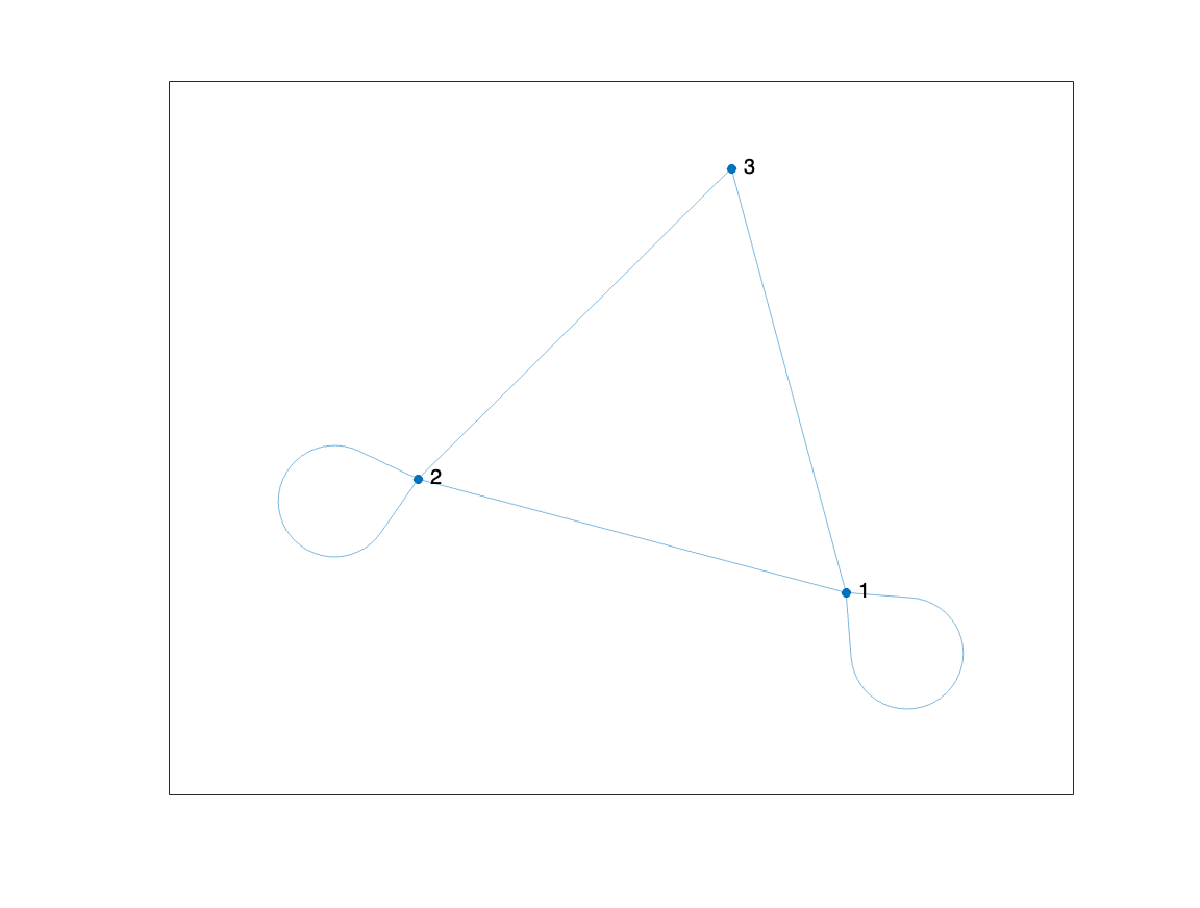
\includegraphics[width=0.5\textwidth]{figure_0}
\end{center}


The input consists of two integer-valued vectors of equal length, from which the graph is built. Each element of each list gives the beginning and ending vertex of the corresponding edge. MATLAB refers to these as the source and target nodes of the given edge. The digraph type differs from the graph type in that each edge is directed from the source to the target. It is digraphs that we use to build quantum graphs.


\begin{matlabcode}
DG= digraph(sources,targets)
\end{matlabcode}
\begin{matlaboutput}
DG = 
  digraph with properties:

    Edges: [5x1 table]
    Nodes: [3x0 table]

\end{matlaboutput}
\begin{matlabcode}
plot(DG)
\end{matlabcode}
\begin{center}
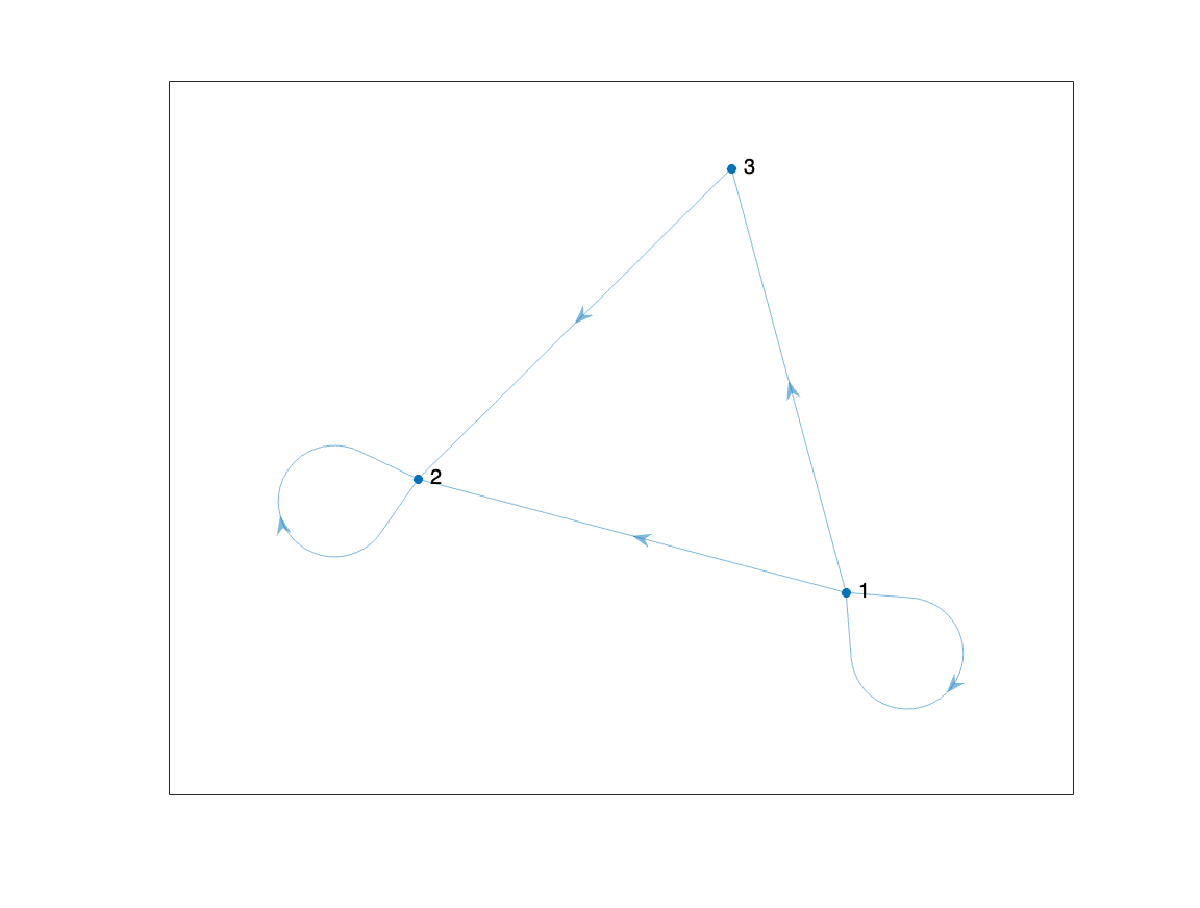
\includegraphics[width=0.5\textwidth]{figure_1}
\end{center}


Note that the two data structures appear the same, but MATLAB does treat them differently and has some distinct commands for dealing with the two of them. For example the function \texttt{degree} calculates the degree of a node in a graph, but does not work on digraph, which has separate functions \texttt{indegree} and \texttt{outdegree} that compute incoming and outgoing degrees. Let's look at the \texttt{Edges} component:


\begin{matlabcode}
DG.Edges
\end{matlabcode}
\begin{matlabtableoutput}
{
\begin{tabular} {|c|c|c|}\hline
\mlcell{ } & \multicolumn{2}{|c|}{\mlcell{EndNodes}} \\ \hline
\mlcell{ } & \mlcell{1} & \mlcell{2} \\ \hline
\mlcell{1} & \mlcell{1} & \mlcell{1} \\ \hline
\mlcell{2} & \mlcell{1} & \mlcell{2} \\ \hline
\mlcell{3} & \mlcell{1} & \mlcell{3} \\ \hline
\mlcell{4} & \mlcell{2} & \mlcell{2} \\ \hline
\mlcell{5} & \mlcell{3} & \mlcell{2} \\ 
\hline
\end{tabular}
}
\end{matlabtableoutput}


Both the \texttt{Edges} and \texttt{Nodes} components are defined as MATLAB \texttt{tables}. At this point the \texttt{Edges} component has one entry called \texttt{EndNodes}. The graph is a purely topological entity. The lengths of the displayed edges are arbitrary. The real usefulness of the data structure is that we can add additional data to both the edges and the nodes. For example we can associate the elements of a vector \texttt{L} to each edge, so long as \texttt{length(L) = length(EndNodes)}.


\begin{matlabcode}
DG.Edges.L=[1;3;5;7;9];
DG.Edges
\end{matlabcode}
\begin{matlabtableoutput}
{
\begin{tabular} {|c|c|c|c|}\hline
\mlcell{ } & \multicolumn{2}{|c|}{\mlcell{EndNodes}} & \mlcell{L} \\ \hline
\mlcell{ } & \mlcell{1} & \mlcell{2} & \mlcell{ } \\ \hline
\mlcell{1} & \mlcell{1} & \mlcell{1} & \mlcell{1} \\ \hline
\mlcell{2} & \mlcell{1} & \mlcell{2} & \mlcell{3} \\ \hline
\mlcell{3} & \mlcell{1} & \mlcell{3} & \mlcell{5} \\ \hline
\mlcell{4} & \mlcell{2} & \mlcell{2} & \mlcell{7} \\ \hline
\mlcell{5} & \mlcell{3} & \mlcell{2} & \mlcell{9} \\ 
\hline
\end{tabular}
}
\end{matlabtableoutput}


The Nodes table is initially empty


\begin{matlabcode}
DG.Nodes
\end{matlabcode}
\begin{matlaboutput}
ans =

  3x0 empty table
\end{matlaboutput}


but we can add data to each node in a similar manner.


\begin{matlabcode}
DG.Nodes.mass = [1;4;9];
DG.Nodes
\end{matlabcode}
\begin{matlabtableoutput}
{
\begin{tabular} {|c|c|}\hline
\mlcell{ } & \mlcell{mass} \\ \hline
\mlcell{1} & \mlcell{1} \\ \hline
\mlcell{2} & \mlcell{4} \\ \hline
\mlcell{3} & \mlcell{9} \\ 
\hline
\end{tabular}
}
\end{matlabtableoutput}


\label{H_B8F3E54F}
\subsection{Graphs MATLAB Can't Work With (version 2017b and earlier).}


Before version 2018a, Matlab's \texttt{digraph }structure could not handle multiple edges sharing the same source and target. Therefore a graph such as the \textit{mandarin graph}, which has two vertices, and three separate edges connecting them cannot be represented.



The following will return an error in MATLAB versions older than 2018a.


\begin{matlabcode}
source=[1 1 1 2]; target=[1 2 2 2];
quantumGraph(source,target,1);
\end{matlabcode}


\label{H_52D3F3BE}
\subsection{Constructing the Quantum Graph}


To create the quantum graph routines, we first created a quantum graph class, which is built on top of the digraph class, and added appropriate data for quantum graph problems:


\begin{matlabcode}
source=[1 1 2];
target=[1 2 2];
L = [2*pi,4, 2*pi];
Phi = quantumGraph(source,target,L);
\end{matlabcode}


There can be other fields associated with the quantum graph but these are either optional fields, or fields set to the default, and must be set in a slightly different way. 



Most of the information is associated with the edges



\texttt{L:} (required)the vector of lengths (if scalar than repeated)



\texttt{nx:} (optional) the number of discretization points on each edge (if scalar then \texttt{nx} is the density of points per unit length and the same value is used on each edge)



\texttt{x} and \texttt{y}: (optional, created if nxVec is set) the independent and dependent variables on each edge. \texttt{y} is set to \texttt{NaN} on initialization. Only created if nxVec specified. If \texttt{length(nxVec)==1}, then it is interpreted as the density of discretizatio points per unit length


\begin{matlabcode}
Phi.Edges
\end{matlabcode}
\begin{matlabtableoutput}
{
\begin{tabular} {|c|c|c|c|c|c|c|c|c|}\hline
\mlcell{ } & \multicolumn{2}{|c|}{\mlcell{EndNodes}} & \mlcell{Weight} & \mlcell{L} & \mlcell{nx} & \mlcell{x} & \mlcell{y} & \mlcell{integrationWeight} \\ \hline
\mlcell{ } & \mlcell{1} & \mlcell{2} & \mlcell{ } & \mlcell{ } & \mlcell{ } & \mlcell{ } & \mlcell{ } & \mlcell{ } \\ \hline
\mlcell{1} & \mlcell{1} & \mlcell{1} & \mlcell{1} & \mlcell{6.2832} & \mlcell{126} & \mlcell{128x1 double} & \mlcell{128x1 double} & \mlcell{0.0499} \\ \hline
\mlcell{2} & \mlcell{1} & \mlcell{2} & \mlcell{1} & \mlcell{4} & \mlcell{80} & \mlcell{82x1 double} & \mlcell{82x1 double} & \mlcell{0.0500} \\ \hline
\mlcell{3} & \mlcell{2} & \mlcell{2} & \mlcell{1} & \mlcell{6.2832} & \mlcell{126} & \mlcell{128x1 double} & \mlcell{128x1 double} & \mlcell{0.0499} \\ 
\hline
\end{tabular}
}
\end{matlabtableoutput}


There are two variables associated to the nodes:



\texttt{y}: the dependent variable



\texttt{robinCoeff}: optional the constant determining the Robin boundary condition used in the Laplacian and in interpolating \texttt{y} from the edges to the nodes. This optional argument defaults to zero, i.e. to Kirchoff/Neuman boundary conditions. May be specified as scalar or vector. At leaf nodes only, Dirichlet boundary conditions can be used. This is specified by a \texttt{NaN}. Specifying \texttt{NaN} at a non-leaf node will return an error.


\begin{matlabcode}
Phi.Nodes
\end{matlabcode}
\begin{matlabtableoutput}
{
\begin{tabular} {|c|c|c|}\hline
\mlcell{ } & \mlcell{robinCoeff} & \mlcell{y} \\ \hline
\mlcell{1} & \mlcell{0} & \mlcell{NaN} \\ \hline
\mlcell{2} & \mlcell{0} & \mlcell{NaN} \\ 
\hline
\end{tabular}
}
\end{matlabtableoutput}


The above quantum graph is suitable for running the secular determinant codes below. This symbolic calculation does not depend on a discretization. However if you want to do numerics, you will need to set up vectors of \textit{x}- and \textit{y}- values along each edge. This involves first defining a vector \texttt{nx} containing the number of x values along each edge (including the endpoints), and then calling the following two routines to set up fields to hold the independent and dependent coordinates. For now, only uniform discretizations are allowed  but in the future we will add support for Chebyshev discretizations. Note that if \texttt{nxvec} is specificed but \texttt{Discretization} is not, then \texttt{Discretization} defaults to \texttt{Uniform}. The general syntax is now



\texttt{dumbbell=quantumGraph(source,target,L,'Key1',value1, 'key2',value2,...)}



The three required input parameters must appear in that order, followed by the optional parameters, specified as key-value pairs, that can appear in any order. The optional arguments, for now, are


\begin{itemize}
\setlength{\itemsep}{-1ex}
   \item{\begin{flushleft} \texttt{nxvec }(associated to edges) \end{flushleft}}
   \item{\begin{flushleft} \texttt{robincoeff }(associated to nodes) \end{flushleft}}
   \item{\begin{flushleft} \texttt{Discretization }(property of graph) \end{flushleft}}
   \item{\begin{flushleft} \texttt{plotCoordinateFcn }(property of graph, allows overloading of \texttt{plot)} \end{flushleft}}
\end{itemize}


In addition, there are methods to add or change these values.  


\begin{matlabcode}
Phi=quantumGraph(source,target,L,...
    'Discretization','Chebyshev',...
    'nxvec',[63 20 63],...
    'plotCoordinateFcn',@dumbbellPlotCoords);
Phi.plot('layout')
\end{matlabcode}
\begin{center}
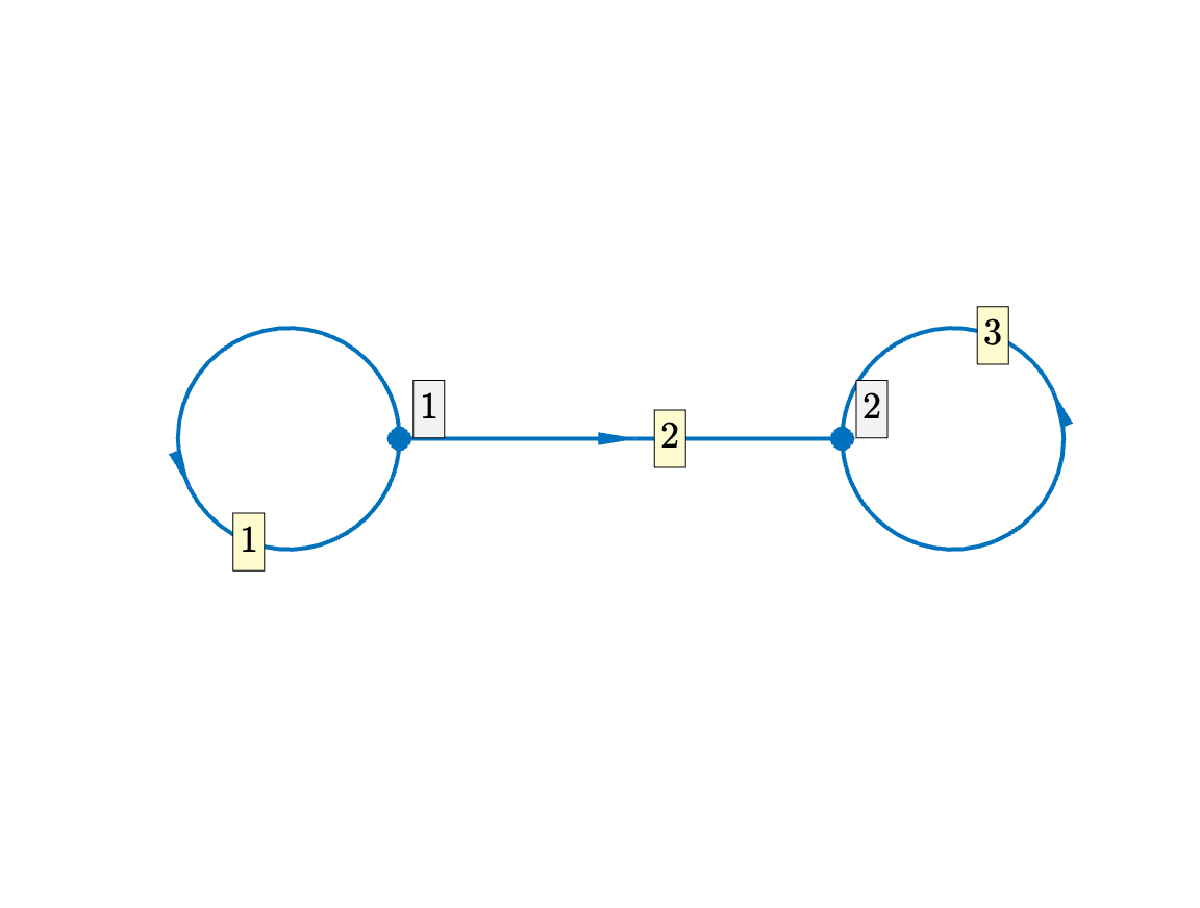
\includegraphics[width=0.5\textwidth]{figure_2}
\end{center}


The final name-value pair specifies the name of a user-defined function that sets up the coordinates and enables the plots of eigenfunctions given below. 



\label{H_8300FE72}
\subsection{Template functions}


For many of our favorite graphs, we have created template functions, which are stored in the directory \texttt{source/templates}. All we need to do to create a dumbbell matrix is to enter


\begin{matlabcode}
Phi = quantumGraphFromTemplate('star');
Phi.plot('layout')
\end{matlabcode}
\begin{center}
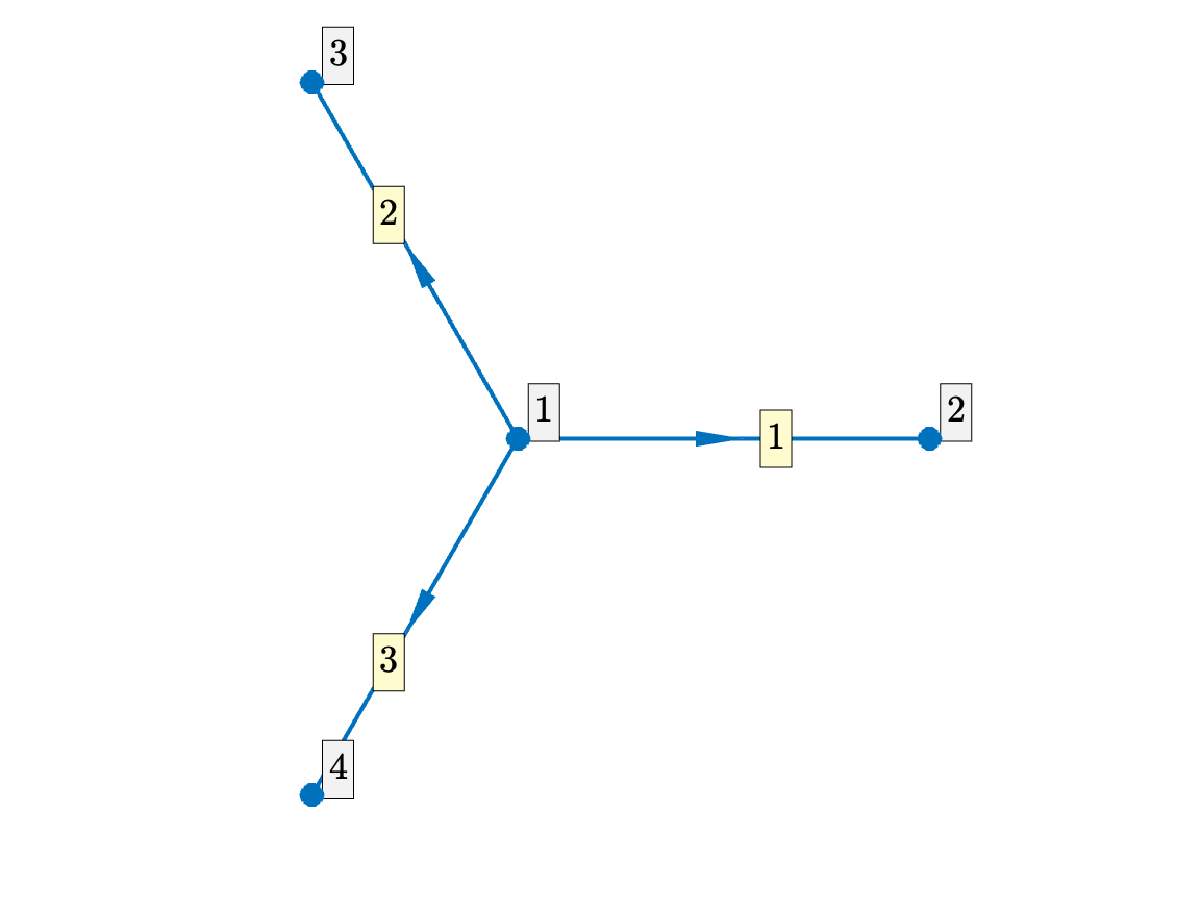
\includegraphics[width=0.35\textwidth]{figure_3}
\end{center}


The template file contains default values for constructing the quantum graph. By default a uniform grid is used with centered difference discretization.  Defaults can be overridden using key-value pairs. Each template constructor contains a program that defines the graph's layout for plotting.



\label{H_527D93F7}
\subsection{Visualizing the quantum graph discretization}


As discussed in the introduction, QGLAB uses a block-matrix formulation to discretize differential equations whose space derivatives are given by Laplacians. This requires the construction of three matrices: the discretized Laplacian, an interpolation matrix, and a vertex condition matrix.  These matrices are constructed directly from the quantum graph object. If a discretization is specified, then they are defined when the quantum graph is initially constructed. 


\label{H_AC72B449}
\matlabheadingthree{Finite Difference}



\begin{matlabcode}
Phi = quantumGraphFromTemplate('dumbbell');
Phi.spy
\end{matlabcode}
\begin{center}
\includegraphics[height=0.4\textwidth]{figure_4}
\includegraphics[height=0.4\textwidth]{figure_5}
\end{center}
\begin{center}
\includegraphics[width=0.5\textwidth]{figure_6}
\end{center}

\label{H_0F37778E}
\matlabheadingthree{Chebyshev}


This, of course, gives higher accuracy at the expense of constructing blockwise-dense matrices.


\begin{matlabcode}
Phi = quantumGraphFromTemplate('dumbbell','Discretization','Chebyshev');
Phi.spy
\end{matlabcode}
\begin{center}
\includegraphics[height=0.4\textwidth]{figure_7}
\includegraphics[height=0.4\textwidth]{figure_8}
\end{center}
\begin{center}
\includegraphics[width=0.5\textwidth]{figure_9}
\end{center}


\label{H_B4668F6C}
\section{Setting up and solving problems on quantum Graphs}

\subsection{A Schrodinger-Poisson problem}


Set up a quantum graph in the form of a dumbbell plus one extra unbounded edge



Solve the vertex-value problem 


\begin{par}
$$\begin{array}{l}
\triangle u-V(x)\,u=f\\
\sum wu^{\prime } ({\vertex_1 })+u({\vertex_1 })=6\\
\sum wu^{\prime } ({\vertex_2 })+u({\vertex_2 })=3\\
u({\vertex_3 })=\sech 2
\end{array}$$
\end{par}


where 


\begin{itemize}
\setlength{\itemsep}{-1ex}
   \item{\begin{flushleft} The potential is $V(x)=\lbrace 2\cos 2x,0,0,0,0\rbrace$ \end{flushleft}}
   \item{\begin{flushleft} The functions on the right-hand-sides are $f=\left\lbrace -\sin 3x,2\cos 2x,-4,-\sin x,\sech x-2\sech^3 x\right\rbrace$on the four edges. \end{flushleft}}
   \item{\begin{flushleft} the edges have lengths $\left\lbrace \pi ,2\pi ,1,2\pi ,2\right\rbrace$. \end{flushleft}}
   \item{\begin{flushleft} The exact solutions on the edges are $\left\lbrace \sin x,\sin^2 x,3x-2x^2 ,1+\sin x,\sech x\right\rbrace$. \end{flushleft}}
\end{itemize}

\matlabheadingthree{Quantum graph definition}



\begin{matlabcode}
s=[1 1 1 2 2];
t=[1 1 2 2 3];
L=[pi 2*pi 1 2*pi 2];
robinCoeff=[1 1 nan];
weight = [1 1 2 1 1];
\end{matlabcode}

\matlabheadingthree{The exact solution}


\begin{matlabcode}
u1=@(x)sin(x);
u2=@(x)sin(x).^2;
u3=@(x)(3*x-2*x.^2);
u4=@(x)(1+sin(x));
u5=@(x)sech(x);
\end{matlabcode}

\matlabheadingthree{The right hand sides}


Edges and nodes


\begin{matlabcode}
f1=@(x)-sin(3*x);
f2=@(x)2*cos(2*x);
f3=-4;
f4=@(x)-sin(x);
f5=@(x)sech(x).*(1-2*sech(x).^2);
nodeData = [8;3;sech(2)];
\end{matlabcode}

\matlabheadingthree{The potential}



\begin{matlabcode}
potentialV = {@(x)(2*cos(2*x)),0,0,0,0};
\end{matlabcode}

\matlabheadingthree{Solve the system }


Define the quantum graph. Use the default value of about 20 discretization points per unit length.


\begin{matlabcode}
Phi=quantumGraph(s,t,L,'RobinCoeff',robinCoeff,'Weight',weight,...
                 'Discretization','Chebyshev');
Phi.addPlotCoords(@poissonExamplePlotCoords);
Phi.addPotential(potentialV);
Phi.plot('layout');
\end{matlabcode}
\begin{center}
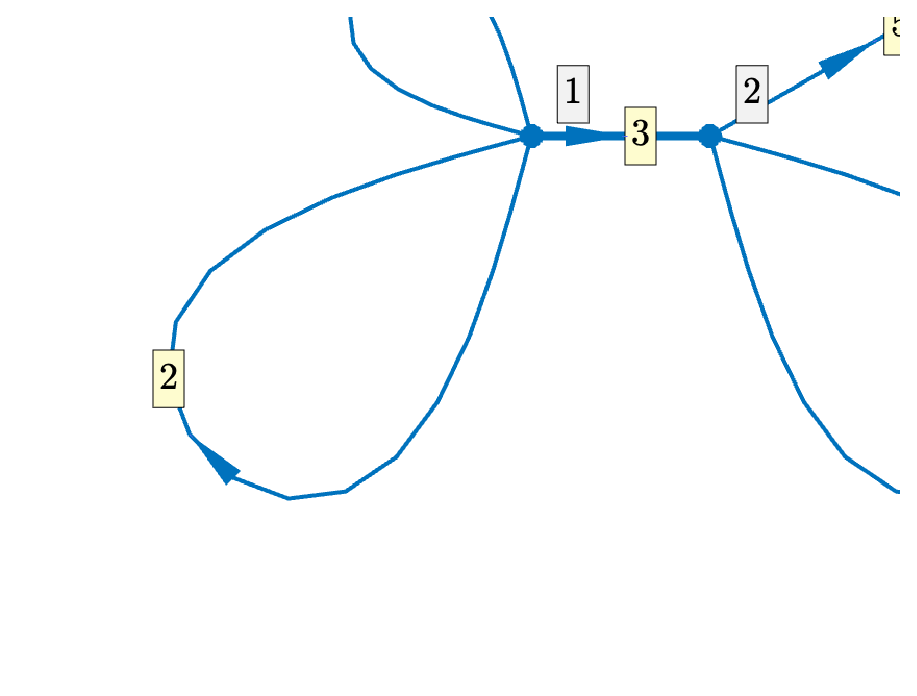
\includegraphics[width=0.5\textwidth]{figure_10}
\end{center}


Set up the exact solution on the edges


\begin{matlabcode}
exactSolution = Phi.applyFunctionsToAllEdges({u1,u2,u3,u4,u5});
\end{matlabcode}


Set up the nonhomogeneous data on the edges


\begin{matlabcode}
edgeData = Phi.applyFunctionsToAllEdges({f1,f2,f3,f4,f5});
\end{matlabcode}


Solve and compute errors


\begin{matlabcode}
numericalSolution = Phi.solvePoisson('edgeData',edgeData,'nodeData',nodeData);
numericalError= Phi.norm(exactSolution-numericalSolution,inf);
fprintf('The maximum error is %0.4d.\n',numericalError)
\end{matlabcode}
\begin{matlaboutput}
The maximum error is 1.0446e-10.
\end{matlaboutput}



Plot the solution


\begin{matlabcode}
Phi.plot(numericalSolution)
\end{matlabcode}
\begin{center}
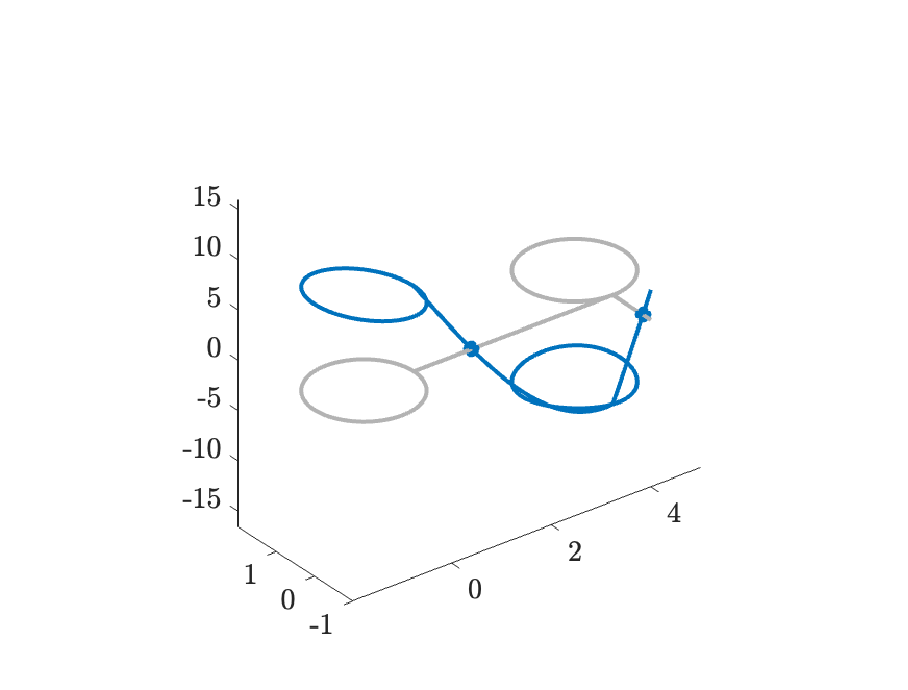
\includegraphics[width=0.5\textwidth]{figure_11}
\end{center}


\label{H_402B04AA}
\subsection{An eigenproblem}


We compute the four eigenvalues closest to zero for the dumbbell quantum graph.


\begin{matlabcode}
Phi=quantumGraphFromTemplate('dumbbell','Discretization','Chebyshev');
[V,lambda]=Phi.eigs(4);
for k=1:4
    figure
    Phi.plot(V(:,k))
    title(sprintf('Eigenfunction %i, $\\lambda = %0.3f$', k, lambda(k)));
end
\end{matlabcode}
\begin{center}
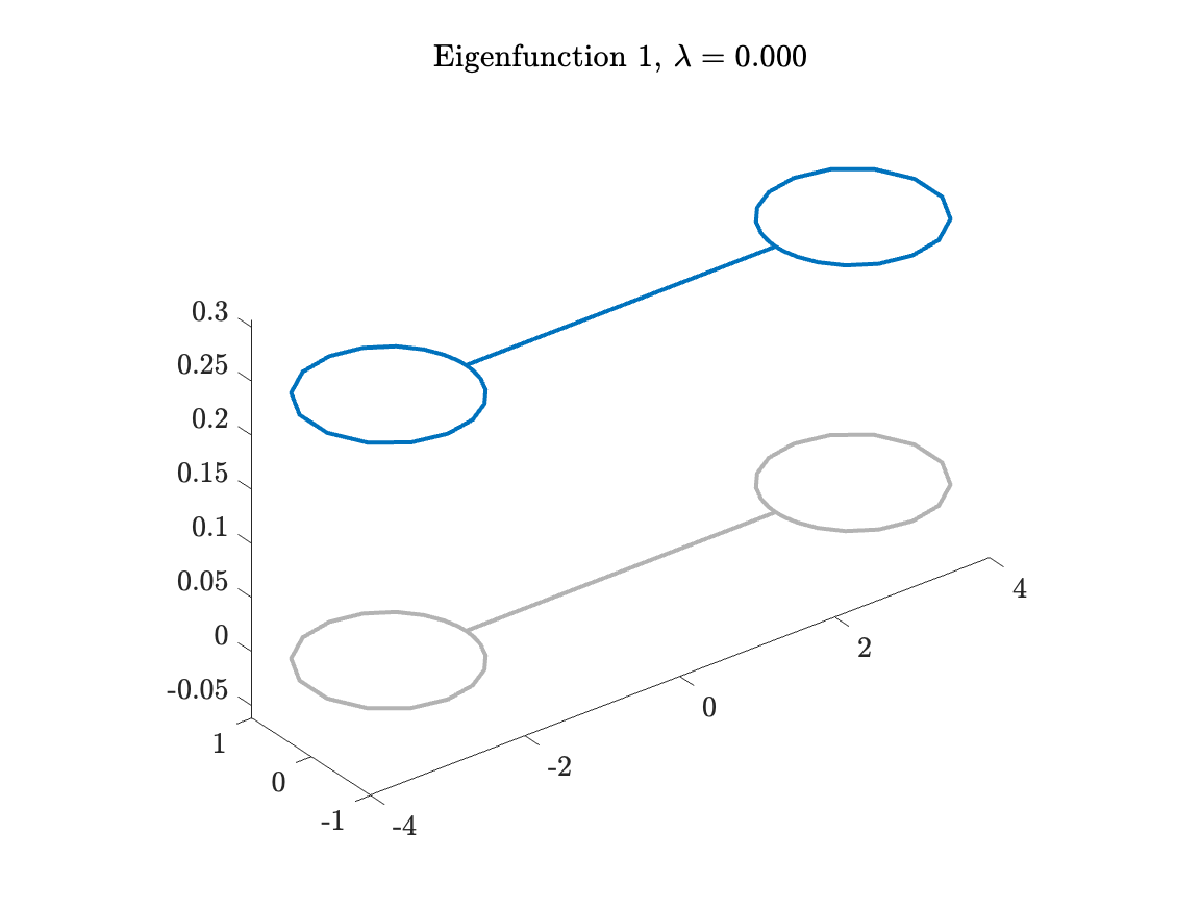
\includegraphics[width=0.4\textwidth]{figure_12}
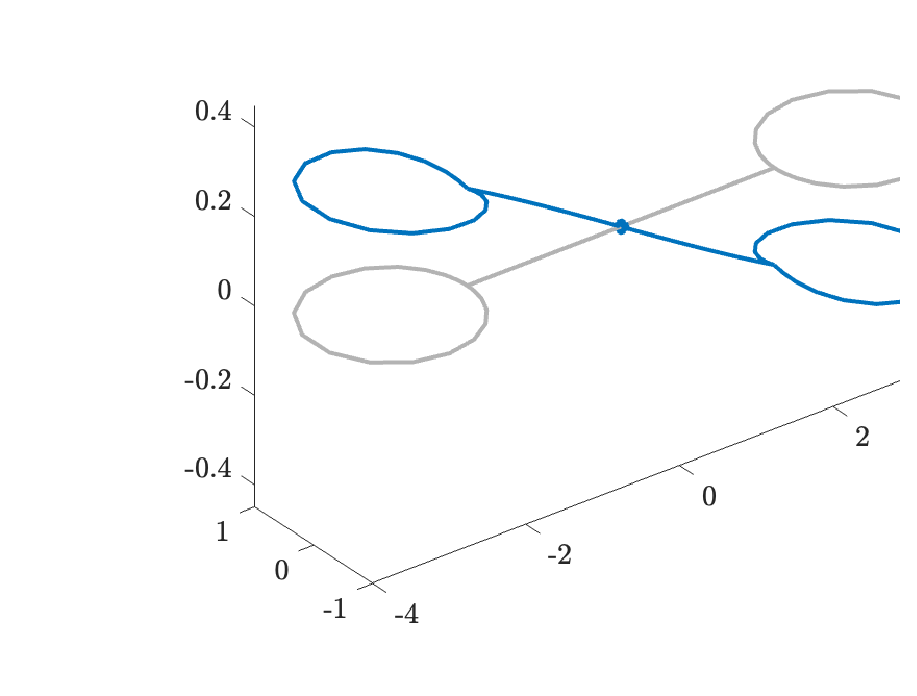
\includegraphics[width=0.4\textwidth]{figure_13}
\end{center}
\begin{center}
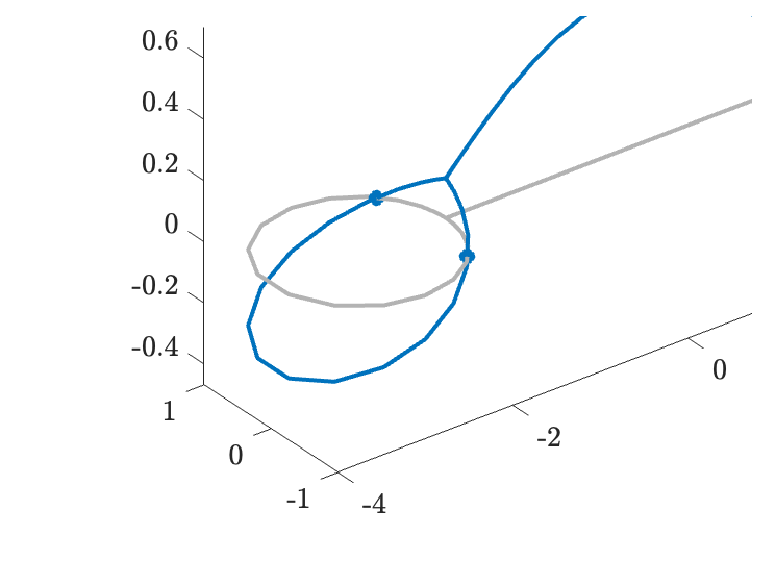
\includegraphics[width=0.4\textwidth]{figure_14}
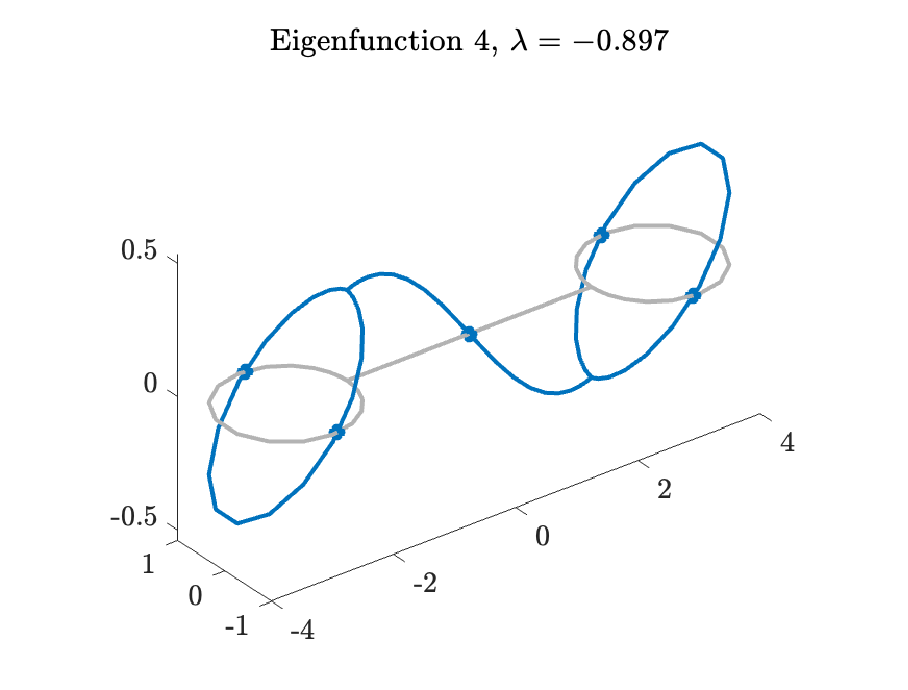
\includegraphics[width=0.4\textwidth]{figure_15}
\end{center}

\label{H_10089249}
\matlabheadingthree{The secular determinant}


The eigenvalues of quantum graph are given by $\lambda =-k^2$ where $k$ is a root of a function called the \textit{secular determinant}. This function is defined by noting that on each edge, the eigenfunction must be a linear combination of $\sin kx$ and $\cos kx$, and attempting to enforce the vertex conditions. The following code constructs the secular determinant as a symbolic expression $f(k)$. 


\begin{matlabcode}
f=secularDet(Phi)
\end{matlabcode}
\begin{matlabsymbolicoutput}
f = 

\hskip1em $\displaystyle -\frac{{\left(\cos \left(2\,\pi \,x\right)-1\right)}\,{\left(4\,\cos \left(4\,x\right)\,\sin \left(2\,\pi \,x\right)-3\,\sin \left(4\,x\right)+5\,\sin \left(4\,x\right)\,\cos \left(2\,\pi \,x\right)\right)}}{4}$
\end{matlabsymbolicoutput}
\begin{matlabcode}
fplot(f,[0 2*pi])
\end{matlabcode}
\begin{center}
\includegraphics[width=0.35\textwidth]{figure_16}
\end{center}
\begin{matlabcode}
k=linspace(0,1);
ff=matlabFunction(f);
fk=ff(k);
\end{matlabcode}


The smallest root is just $k=0$. Find the next three and see that they agree with the eigenvalues to all digits shown


\begin{matlabcode}
guesses=find(fk(1:end-1).*fk(2:end)<0);
fprintf('Numerical  Analytical')
\end{matlabcode}
\begin{matlaboutput}
Numerical  Analytical
\end{matlaboutput}
\begin{matlabcode}
for i=1:3
    kstar=fzero(ff,k(guesses(i)));
    fprintf('%2.5f    %2.5f\n',lambda(i+1),-kstar^2)
end
\end{matlabcode}
\begin{matlaboutput}
Numerical  Analytical
-0.05857    -0.05857
-0.42970    -0.42970
-0.89706    -0.89706
\end{matlaboutput}


\subsection{Drawing a bifurcation diagram}


This code draws the bifurcation diagram from~\cite[Fig. 3.3]{Goodman:2019go} plus some extra branches to show how the code works.



\matlabheadingthree{Construct the quantum graph and find the first few eigenfunctions}

The program requires a pair of template files to construct the quantum graph and lay out the plotting. Here, we use the \texttt{dumbbell} template. Each time the code runs, it creates a new numbered folder under \texttt{data/dumbbell}.

\begin{matlabcode}
tag='dumbbell';
L = [2*pi 4 2*pi];
nxvec=6;
Phi=quantumGraphFromTemplate(tag,'LVec',L,'nX',nxvec,'discretization','Uniform');
dataDir = makeContinuationDirectory(Phi,tag);
\end{matlabcode}
\begin{matlaboutput}
Created directory data/dumbbell/182.
\end{matlaboutput}

I've run this program many times, so the data is saved in folder number 182.

\matlabheadingthree{Compute and save some eigenfunctions}

I instruct it to save four multiplicity-one eigenfunctions and one multiplicity-two eigenfunction. This lets us continue solutions from the linear limit.

\begin{matlabcode}
nToPlot=4;
nDoubles=1;
saveEigenfunctions(Phi,tag,dataDir,nToPlot,nDoubles);
\end{matlabcode}

\matlabheadingthree{Define the cubic nonlinearity and save it to the data directory. }


This must be a symbolic function of a single variable \texttt{z}.


\begin{matlabcode}
syms z
f = 2*z^3;
fcns = saveNLSFunctionsGraph(dataDir,Phi,f);
\end{matlabcode}


\matlabheadingthree{Compute branches that are continuation of the three least oscillatory eigenfunctions}

\begin{itemize}
\setlength{\itemsep}{-1ex}
   \item{\begin{flushleft} The function \texttt{continuerSet} acts like the MATLAB functions \texttt{odeset} and \texttt{optimset.} It sets a number of options that are used by the continuation programs \end{flushleft}}
   \item{\begin{flushleft} The function \texttt{continueFromEig} continues a branch from the linear limit of an eigenfunction computed in the previous step \end{flushleft}}
\end{itemize}

\begin{matlabcode}
options=continuerSet([],'LambdaThresh',-3,'NThresh',9,'plotFlag',false,'minNormDelta',1e-3);
branch1=continueFromEig(dataDir,1,options);
\end{matlabcode}
\begin{matlaboutput}
N threshold 9.0 crossed.
Branch number 1.
Data saved to directory data/dumbbell/182/branch001.
Branching Bifurcation at solution number 6.
Branching Bifurcation at solution number 9.
Branching Bifurcation at solution number 12.
Branching Bifurcation at solution number 14.
\end{matlaboutput}
\begin{matlabcode}
branch2=continueFromEig(dataDir,2,options);
\end{matlabcode}
\begin{matlaboutput}
Lambda threshold -3.0 crossed.
Branch number 2.
Data saved to directory data/dumbbell/182/branch002.
No branching bifurcations found.
\end{matlaboutput}
\begin{matlabcode}
branch3=continueFromEig(dataDir,3,options);
\end{matlabcode}
\begin{matlaboutput}
N threshold 9.0 crossed.
Branch number 3.
Data saved to directory data/dumbbell/182/branch003.
No branching bifurcations found.
\end{matlaboutput}


\matlabheadingthree{Compute some branches that bifurcate from this first branch}

\begin{itemize}
\setlength{\itemsep}{-1ex}
   \item{\begin{flushleft} The function \texttt{continueFromBranchpoint} continues a branch from the first branching bifurcation point. Since this is a symmetry-breaking bfirucation, we only need to continue in one direction, the branch stored in \texttt{branch1} at bifurcation location 1  \end{flushleft}}
\end{itemize}

\begin{matlabcode}
location=1;
direction=1;
branch4=continueFromBranchPoint(dataDir,branch1,location,direction,options);
\end{matlabcode}
\begin{matlaboutput}
Lambda threshold -3.0 crossed.
Branch number 4.
Data saved to directory data/dumbbell/182/branch004.
No branching bifurcations found.
\end{matlaboutput}


\begin{itemize}
\setlength{\itemsep}{-1ex}
   \item{\begin{flushleft} The function \texttt{continueFromBranchpoint} continues a branch from the first branching bifurcation point. Since this is a transcritical bfirucation, we need to continue in both directions, the branch stored in \texttt{branch1} at bifurcation location 2 \end{flushleft}}
\end{itemize}

\begin{matlabcode}
location=2;
direction=1;
branch5=continueFromBranchPoint(dataDir,branch1,location,direction,options);
\end{matlabcode}
\begin{matlaboutput}
Lambda threshold -3.0 crossed.
Branch number 5.
Data saved to directory data/dumbbell/182/branch005.
Branching Bifurcation at solution number 21.
\end{matlaboutput}
\begin{matlabcode}
location=2;
direction=-1;
branch6=continueFromBranchPoint(dataDir,branch1,location,direction,options);
\end{matlabcode}
\begin{matlaboutput}
Lambda threshold -3.0 crossed.
Branch number 6.
Data saved to directory data/dumbbell/182/branch006.
No branching bifurcations found.
\end{matlaboutput}


\matlabheadingthree{Compute a branch that bifurcates from the third branch}


Continues from the branch stored in \texttt{branch5} from the bifurcation point 1


\begin{matlabcode}
location=1;
direction=1;
branch7=continueFromBranchPoint(dataDir,branch5,location,direction,options);
\end{matlabcode}
\begin{matlaboutput}
Lambda threshold -3.0 crossed.
Branch number 7.
Data saved to directory data/dumbbell/182/branch007.
No branching bifurcations found.
\end{matlaboutput}


\matlabheadingthree{Compute a large-amplitude solution, save it to a file, and compute its continuation}


This seeds a standing wave with large frequency, localized and with positive amplitudes on edges 1 and 2.


\begin{matlabcode}
Lambda0=-4;
edges=[1 2];
signs=[1 1];
filenumber=saveHighFrequencyStandingWave(dataDir,Lambda0,edges,signs);
\end{matlabcode}
\begin{matlaboutput}
File saved to data/dumbbell/182/savedFunction.001.
File number is 1. 
\end{matlaboutput}
\begin{matlabcode}
options=continuerSet(options,'LambdaThresh',-4.1,'NThresh',9);
direction=-1;
branch8=continueFromSaved(dataDir,filenumber,direction,options);
\end{matlabcode}
\begin{matlaboutput}
N threshold 9.0 crossed.
Branch number 8.
Data saved to directory data/dumbbell/182/branch008.
No branching bifurcations found.
\end{matlaboutput}
\begin{matlabcode}
bifurcationDiagram(dataDir)
\end{matlabcode}
\begin{center}
\includegraphics[width=0.5\textwidth]{figure_17}
\end{center}


\matlabheadingthree{Plot some solutions}


The fifteenth computed solution on branch 4:


\begin{matlabcode}
plotSolution(dataDir,branch4,15)
\end{matlabcode}
\begin{center}
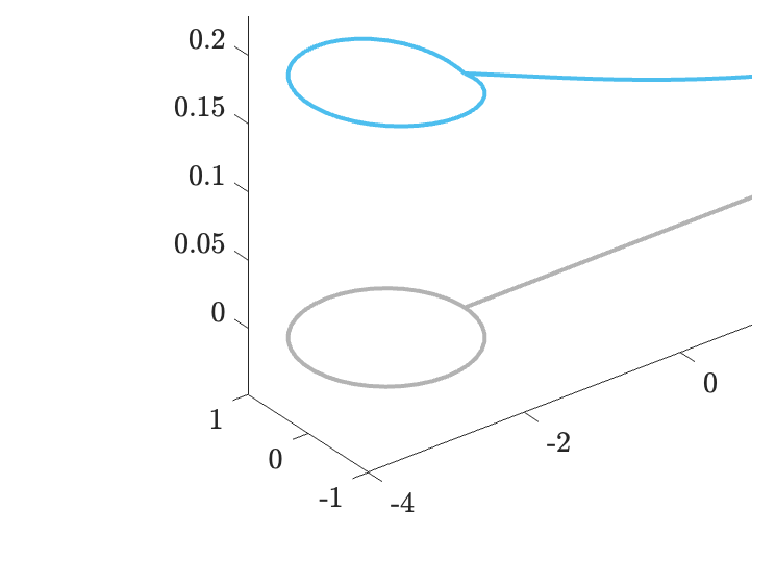
\includegraphics[width=0.5\textwidth]{figure_18}
\end{center}



The last computed solution on branch 8:


\begin{matlabcode}
plotSolution(dataDir,branch8,'last')
\end{matlabcode}
\begin{center}
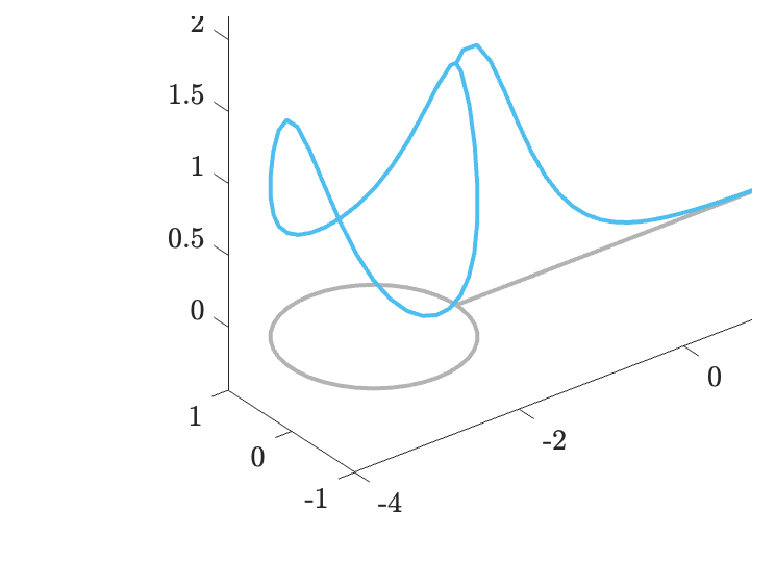
\includegraphics[width=0.5\textwidth]{figure_19}
\end{center}


\subsection{Heat flow on a dumbbell graph}


In this example, we adapt a standard time-stepper, the Crank-Nicholson method to the block matrix formulation. We solve the heat equation $u_t =\triangle u$ on a dumbbell graph.



The standard Crank-Nicholson method with time step $h$ is:



$\left(I-\frac{h}{2}\triangle \right)u_{k+1} =\left(I+\frac{h}{2}\triangle \right)u_k$.



We must modify that to ensure that $u_{k+1}$ satisfies the discrete vertex conditions. In the notation of the paper we let


\begin{par}
$$L_- =\binom{P_{{\mathrm{i}\mathrm{n}\mathrm{t}}} -\frac{h}{2}L_{{\mathrm{i}\mathrm{n}\mathrm{t}}} }{M_{{\mathrm{V}\mathrm{C}}} }\;\textrm{and}\;L_+ =\binom{P_{{\mathrm{i}\mathrm{n}\mathrm{t}}} +\frac{h}{2}L_{{\mathrm{i}\mathrm{n}\mathrm{t}}} }{0}$$
\end{par}


and then iterate $L_- u_{k+1} =L_+ u_k$. The matrices are defined blockwise, with the upper blocks represent the differential equation on the edges' interiors and the bottom blocks enforce the vertex conditions.


\matlabheadingthree{Set up the graph and the initial condition}



\begin{matlabcode}
Phi=quantumGraphFromTemplate('dumbbell');
f0=@(x)(2-2*cos(x-pi/3));
f1=1;
f2=@(x)cos(x);
y=Phi.applyFunctionsToAllEdges({f0,f1,f2});
totalHeatInitial = Phi.integral(y);
figure;Phi.plot(y);
\end{matlabcode}
\begin{center}
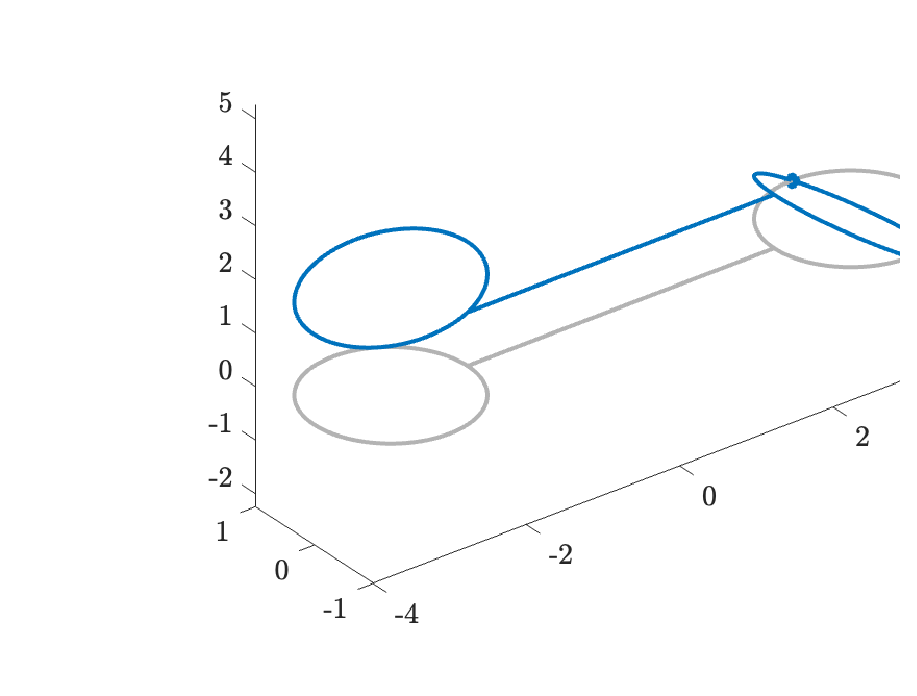
\includegraphics[width=0.5\textwidth]{figure_20}
\end{center}
\begin{matlabcode}

\end{matlabcode}

\matlabheadingthree{Set up the time stepping}



\begin{matlabcode}
h=0.01;
tFinal=10;
nStep=tFinal/h;
\end{matlabcode}

\matlabheadingthree{Set up the evolution matrices}



\begin{matlabcode}
Lint=Phi.wideLaplacianMatrix;
Pint=Phi.interpolationMatrix;
Lplus=Phi.extendWithZeros(Pint+h/2*Lint);
Lminus=Phi.extendWithVC(Pint-h/2*Lint);
\end{matlabcode}

\matlabheadingthree{Evolve  the solution}



\begin{matlabcode}
keepCount=1;
for k=1:nStep
    y = Lplus*y;
    y = Lminus\y;
end
totalHeatFinal = Phi.integral(y);
figure;Phi.plot(y);
\end{matlabcode}
\begin{center}
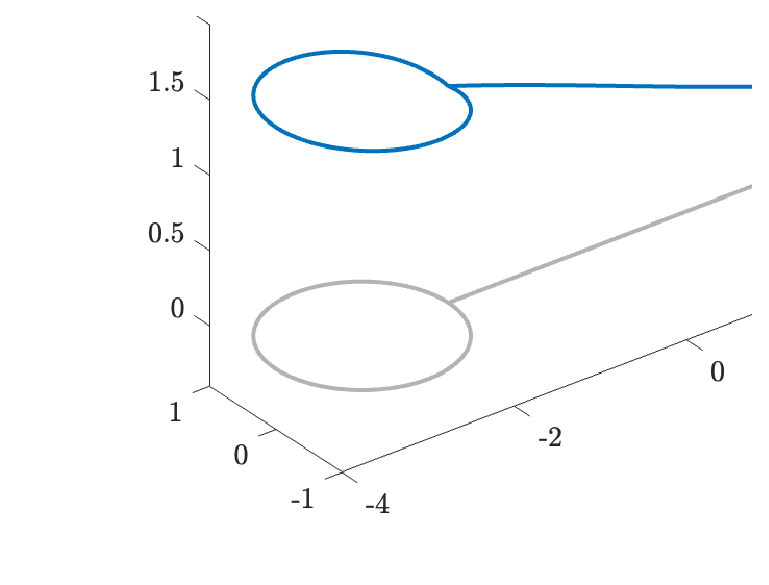
\includegraphics[width=0.5\textwidth]{figure_21}
\end{center}

\matlabheadingthree{Show that the total heat is conserved to many digits}



\begin{matlabcode}
fprintf('Change in heat is %0.2e.\n',totalHeatFinal-totalHeatInitial);
\end{matlabcode}
\begin{matlaboutput}
Change in heat is -1.58e-12.
\end{matlaboutput}


\subsection{KPP evolution on a honeycomb}


We solve the KPP equation $u_t =\mu \triangle u+u(1-u)$ on a honeycomb graph. Here, we evolve the approximate solution using the QGLAB function \texttt{qgdeSDIRK443}. This implements an implicit-explicit (IMEX) Runge-Kutta method due to Nørsett. Such methods are used to handle stiff terms (those coming from the Laplacian) implicitly while using an explicit method to march forward the nonlinear terms so that the implicit part remains linear and no Newton iterations are required. Due to the block-matrix formulation in QGLAB, the explicit part of the method becomes implicit, but the only implicit terms enforce the vertex conditions and are linear.

\begin{matlabcode}
Phi = hexOfHexes("cellsPerSide",4,"nx",32);
\end{matlabcode}


\matlabheadingthree{Define and plot the initial conditions }


We choose an initial condition which is a Gaussian based on the physical coordinates of the points on the graph. This graph has 132 edges and we center the initial condition on the center of edge $\edge_{53}$.


\begin{matlabcode}
centerEdge=53;
spot=round(Phi.nx(centerEdge)/2);
X1=Phi.Edges.x1{centerEdge}(spot);
X2=Phi.Edges.x2{centerEdge}(spot);
f0 = @(x1,x2)exp(-(x1-X1).^2-(x2-X2).^2)/2;
u0 = Phi.applyGraphicalFunction(f0);
Phi.pcolor(u0)
\end{matlabcode}
\begin{center}
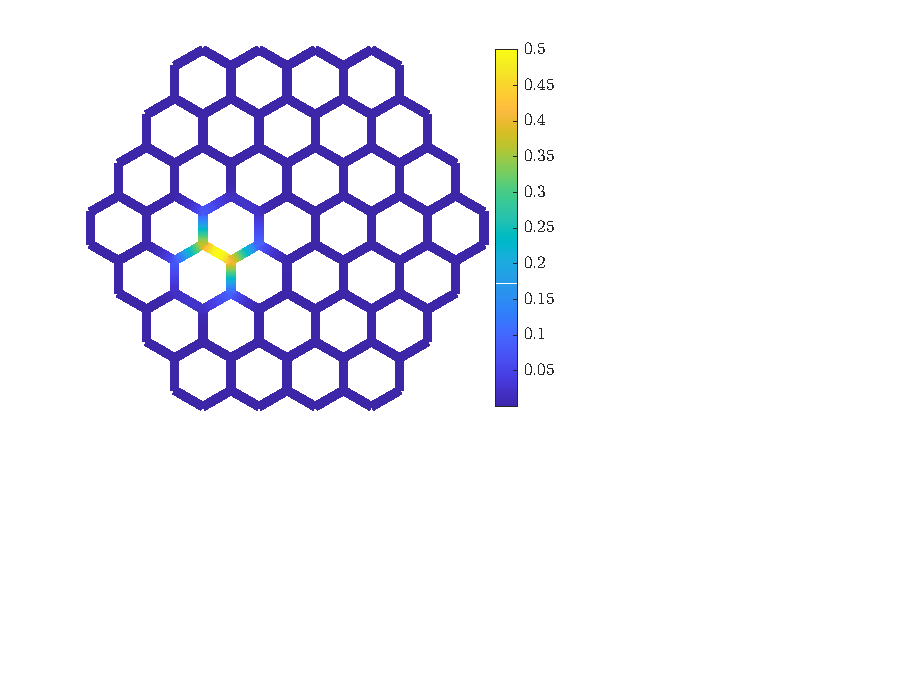
\includegraphics[width=0.35\textwidth]{figure_22}
\end{center}


\matlabheadingthree{Function Definition and Time evolution}

\begin{par}
$$f(t,u)=\mu \triangle u+F(t,u)$$
\end{par}

\begin{matlabcode}
mu = 0.1;
F =@(z) z.*(1-z);
tFinal = 12;
dt = 0.1;
[t,u] = Phi.qgdeSDIRK443(mu,F,tFinal,u0,dt,'nSkip',10);
Phi.pcolor(u(:,end))
\end{matlabcode}
\begin{center}
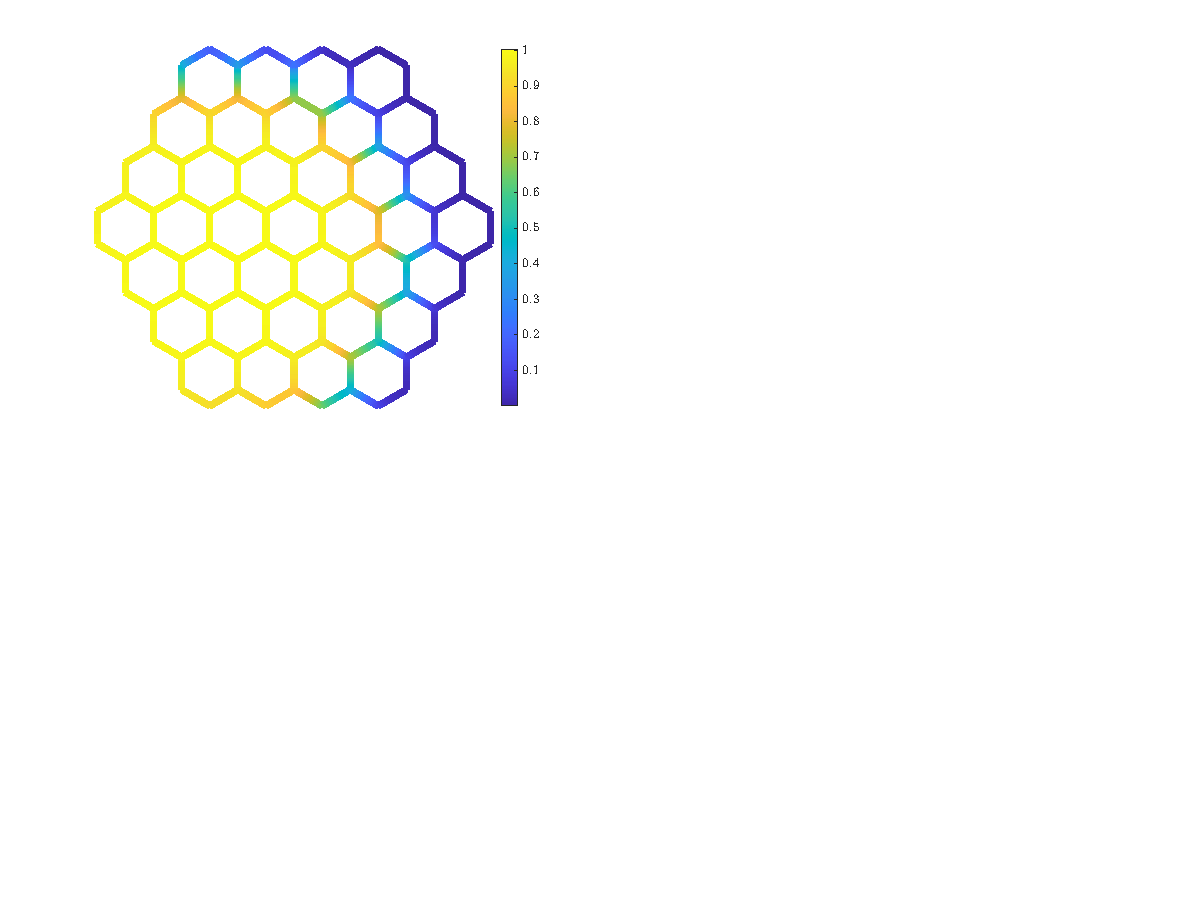
\includegraphics[width=0.35\textwidth]{figure_23}
\end{center}

\bibliography{references.bib}
\bibliographystyle{abbrv}

\end{document}
